This chapter identifies an intersectional space across the described technologies, and proposes a valuable and novel software stack, which can enable exploration  and product development. It is useful to briefly look recap the book and the conclusions we have drawn so far.

\section{Summary TL;DR}
\label{sec:tldr}
\begin{itemize}
\item There may be an inflection point in the organisational topology of the internet because of trust abuses by the incumbent providers. This has been calling itself Web3, but the moniker is fraught with problems and somewhat meaningless. The drivers are real.
\item `The Metaverse' is coming, in some form, at some point. Everyone is positioning in case it's ``soon''.
\item It's not at all clear what it is, or if people want it, but the best emergent narrative seems to be ``digital society'' and that obviously should not be dismissed lightly.
\item From a business perspective metaverse is the worst of the remote collaboration tool-kits, and undermines flow, productivity, and interpersonal trust.
\item Metaverse is probably technology for technologies sake at this time, but it's a strong attempt, and the investment is real. Digital society is more tangible but less hyped.
\item Excluding Facebook/Meta a lot of the investment is coming from the recent Web3 speculative bubble, who have a parallel and intersectional metaverse narrative based around distributed financial tooling and digital assets. 
\item Industry has noted the risk, and failures of Meta in this domain, and have latched onto "open metaverse" as a narrative, to de-risk their interest. The current open metaverse is muddy and confused.
\item Anything from a multi-million pound XR studio screen, to a speech audio system, can be a digital society interface. 
\item AI \& machine learning is further blurring these boundaries. A better term for AI/ML is `supported creativity' and/or `supported intelligence'.
%\item Constraints (metaverse schema) which are crafted in response to the use case, the interface, and the audience, is where challenges are most profound. This is an opportunity.
\item Trust, accessibility, governance, and safeguarding, are hard problems, and made more complex by unrecorded social flow in immersive social VR.
\item Industry seem to be missing the point; that open metaverse should mean open source metaverse. There are some options, but they are under developed. This is an opportunity.
%\item There's a bunch of start-ups and options, interesting research, and some adoption, but scaling is very hard in the face of tepid consumer interest. We need to be driven by use cases.
\item There is genuine, undeniable interest in digital scarcity. The ownership of digital goods seems natural to younger, digitally native users. This is serviced already by various (gaming) platforms, but they are all isolated ecosystems.
\item Uniting these attempts, with portable (transferable) ``goods'' across digital society likely requires a global digital ledger (blockchain), indeed this is the basis of the competing Web3 interpretation. Crypto is igniting imagination on this topic, and is seeing adoption both inside out outside of the metaverse contexts.
\item Crypto is a nightmare; rife with scams, poor technology choices, limited life, and incorrect assumptions. The only thing blockchain/crypto can do well is ``money like networks'', which is a cornerstone of human interaction, and the killer application.
\item Representations of dollars and pounds can ride securely on top of such networks as stablecoins, and this is getting easier to integrate, though there are risks.
\item It's unclear which technology will win, if any, but since the tools exist now they can be integrated now.
\item Legislative and cultural headwinds are significant. There might be no opportunity here in the end, though ``rough game theory'' supports the attempt.
\item Money, digital asset, identity, and thereby trust, can already be mediated by the Bitcoin network, even without using Bitcoin the asset. This is an opportunity.
%\item Digital ownership is nearly possible at scale, low cost, and minimal environmental impact, with the Bitcoin network. This is an opportunity.
\item A topologically flat, inclusive, permissionless, open metaverse, with economically empowered ML and AI actors, which can mediate governance issues, transparently, according to well constructed custom schemas, between cryptographically verifiable economic users (human or AI) is an opportunity.
\item New open source `supported creativity' tooling from StabilityAI potentially removes many of the problems with accessibility, creativity, language barriers, safeguarding, and governance. This is a huge opportunity.
\item Using new image generation ML it may be possible to build a new kind of collaborative global teams for virtual production, ideating in simplistic immersive spaces while instantly creating demonstrable in camera scenes which can be stylised using verbal commands in real-time.
\item Such teams would could be far more ad-hoc by leveraging the designs outlines in this book. This kind of genuine digital society use case is something sorely lacking in large scale attempts such as Meta Horizons.
\item Supporting collaborative working in social VR need not be complex or large scale, but it must be secure, trusted, and task appropriate. This is the reason for this book and product stack.
\end{itemize}



\section{Software stack}
This section needs building out to describe the stack and the choices made, but can be seen in Figure \ref{fig:pyramind} and Figure \ref{fig:highlevelstack}.

\begin{figure*}[ht]\centering 	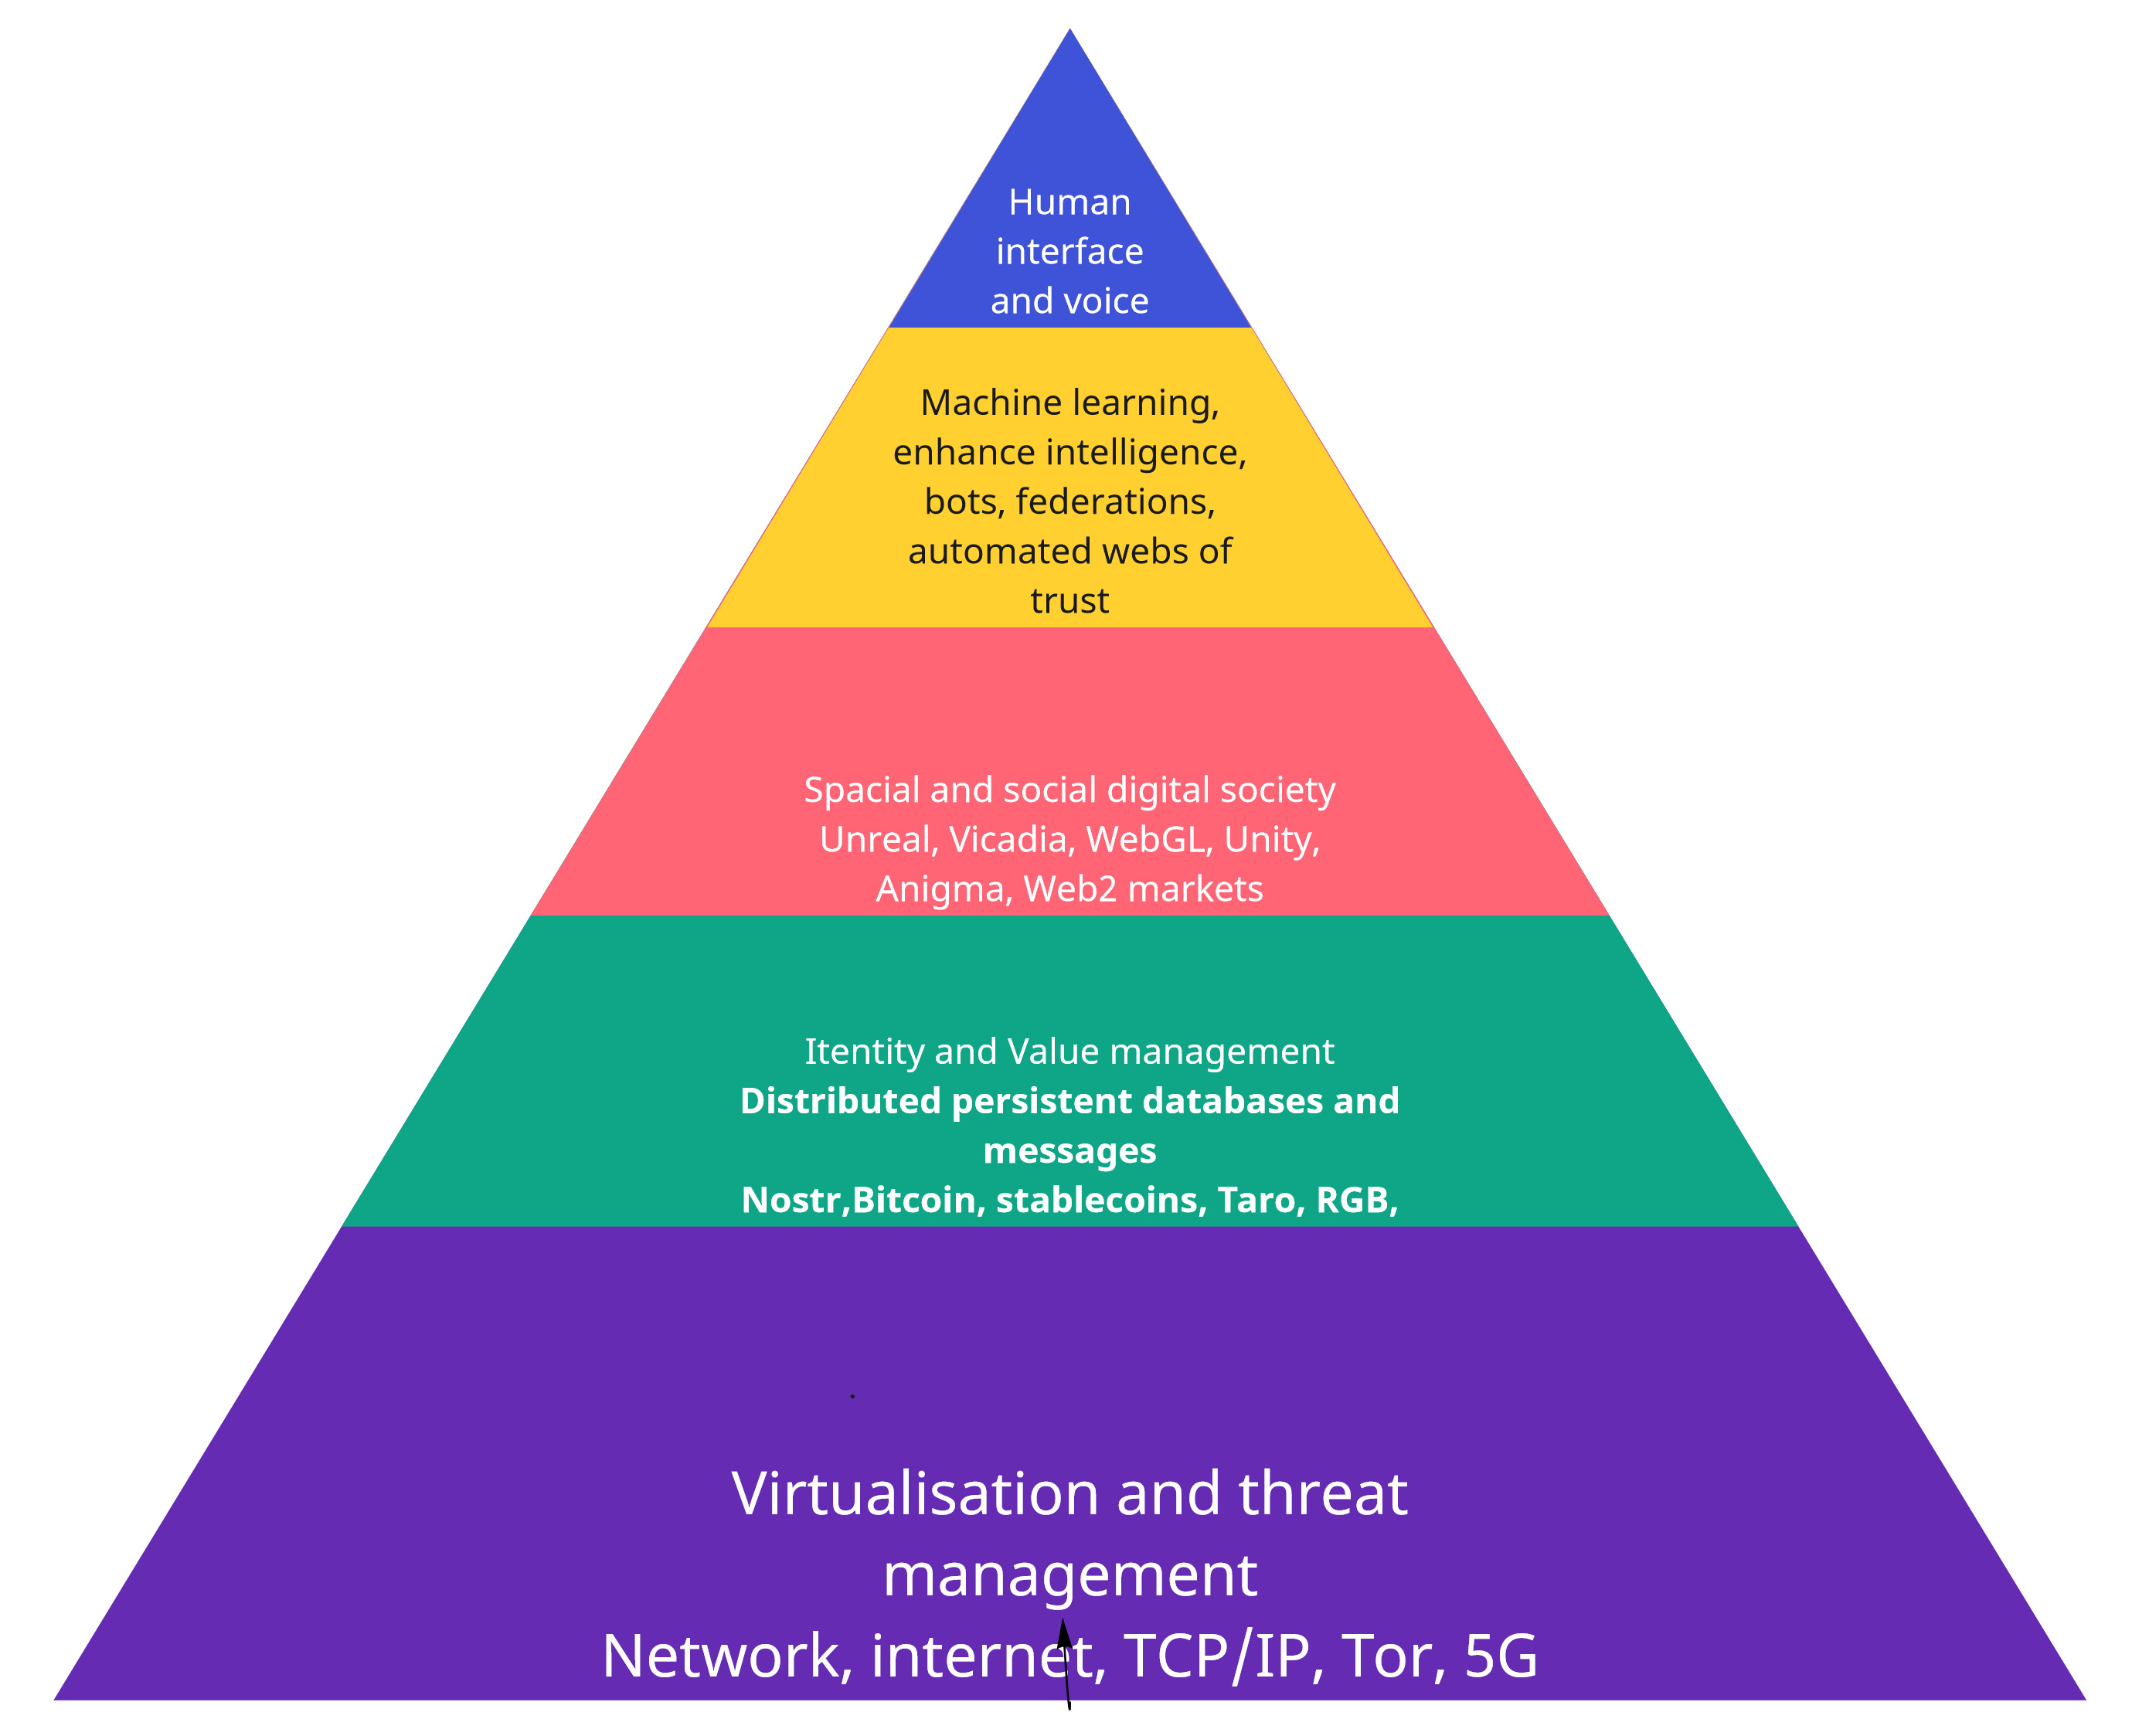
\includegraphics[width=\linewidth]{pyramid}
	\caption{Pyramid showing the components for sats, stablecoins on lightning, asssets, and trust}
	\label{fig:pyramind}
\end{figure*}

\begin{figure*}[ht]\centering 	\includegraphics[width=\linewidth]{highlevelstack}
	\caption{High level overview showing the components for sats, stablecoins on lightning, asssets, and trust}
	\label{fig:highlevelstack}
\end{figure*}

\section{Pathway \& telepresence}
Designing open federated metaverse from a 25 year research foundation
There are serious and under discussed natural social constraints on group behaviours, and these translate into social VR. For instance the ideal meeting size is 6, and this is naturally established in work settings. This has not translated into a metaverse setting where dozens of people routinely crash across one another. In the context of supporting a creative “backstage” world where set planning, production shots, etc can be discussed we believe we have solutions which will get the best out of distributed teams of film-makers.
Leveraging the world's most powerful decentralised computing network to create 
scale and security without high cost
The Bitcoin network is more than just a speculative money like asset, it is the most secure distributed computing system ever built. We can jump on the back of this at almost no cost to enable scale for transfer of value, trust, and digital assets of provenance.
Cryptographically assured end points
With the cryptography tools provided through integration of the Bitcoin network we can also use non-blockchain based secure messaging, and identity proofs. 
Micro transactions in collaborative spaces
New tooling the space allows fractions of a pound or dollar to be exchanged between parties across the world. This means that work can be paid “by the second” both inside and outside of the metaverse. This radically improves creative microtask workflows.
World leading open source machine learning and bot architectures
By integrating Stablity AI tools for image generation, video processing, natural language, and speech to text / text to speech we hope to reduce friction within the backstage worlds.
Creating a narrative arrow from a remote director/producer/DP, through a VP screen into a shoot, and back into a persistent metaverse shared with the public
By linking across these new systems with world class telepresence research we hope to use a single digital context to support senior stakeholders, creatives, technical teams, and the wider public.
New paths to monetisation and digital ownership
This unified digital back end is optimised for flows of money, trust, and digital objects. This is a new area for VP.
Current workstreams:
\begin{itemize}
\item Storyboarding with text2img and dreambooth to add talent and costume ideas before meeting up, as demonstrated in this document \cite{ruiz2022dreambooth}.
\item Collaborative, self hosted, high speed, low detail, economically and cryptographically enabled set design spaces, with near instant language translation (speech to text an speech to speech). Micropayment for cheap international labour. Technology agnostic. Use the screen, audio only, compressed video dial-in, headsets, tablet rendering: (this book).
\item High end telepresence \cite{Roberts2015, OHare2018, Fairchild2017, OHare2016} into the studio/shoot from the virtual set, allowing high value stakeholders to be `present` on set as virtual collaborants with spatial descrimination allowing directional queues. This involved real time human capture like moveAI or the expensive rigs with DSLRs.
\item Novel render pipeline for fast turnaround of final look and feel, taking the rough scene and applying img2img ML with the kind of interframe consistency we are starting to see from the video projects \cite{anonymous2023phenaki}.
\item Text to model pipeline for interactively building key elements with senior stakeholders, pushed from post ideation the the  pre-shoot Unreal content creation \cite{poole2022dreamfusion}.
\item All assets switch over to Unreal metaverse and become consistent (optimised) digital set which can be visited by stakeholders, funders, VIPs etc. Public can visit later for a fee? Digital assets can be bought from the set.
\end{itemize}

\section{Novel VP render pipeline}
Putting the ML image generation on the end of a real-time tracked camera render pipeline might remove the need for detail in set building. To describe how this might work, the set designer, DP, director, etc will be able to ideate in a headset based metaverse of the set design, dropping very basic chairs, windows, light sources whatever. There is -no need- then to create a scene in detail. If the interframe consistency (img2img) can deliver then the output on the VP screen can simply inherit the artistic style from the text prompts, and render production quality from the basic building blocks. Everyone in the set (or just DP/director) could then switch in headset to the final output and ideate (verbally) to create the look and feel (lens, bokeh, light, artistic style etc). This isn’t ready yet as the frames need to generate much faster (100x), but it’s very likely coming in months not years. This ``next level pre-vis'' is being trailed by Pathway in the Vircadia collaborative environment described in this book, and can be seen illustrated in Figure \ref{fig:vircadiasd}.\par
\begin{figure}[ht]\centering 	\includegraphics[width=\linewidth]{vircadiasd}
	\caption{Top panel is a screen grab from Vircadia and the bottom panel is a quick pass through img2img from Stable Diffusion.}
	\label{fig:vircadiasd}
\end{figure}

This can be done now through the use of camera robots. A scene can be built in basic outline, the camera tracks can be encoded into the robot, and the scene can be rapidly post rendered by Stability with high inter frame consistency.\par
With the help of AI projects such as \href{https://nv-tlabs.github.io/LION/}{LION} it may be possible to pass simple geometry and instructions to ML systems which can create complex textured geometry back into the scene.
\begin{figure}[ht]\centering 	\includegraphics[width=\linewidth]{robotvp}
	\caption{Robot VP}
	\label{fig:robotvp}
\end{figure}

\section{Money in metaverses}
\subsubsection{Global collaboration and remuneration}
In the book ``Ghosts of my life'' \cite{fisher2014ghosts} Fisher asserts that there has been a slowing, even a `cancellation' of creative progress in developed societies, their art, and their media. His contention is that neoliberalism itself is to blame. He says\\
\textit{``It is the contention of this book that 21st-century culture is marked by the same anachronism and inertia which afflicted Sapphire and Steel in their final adventure. But this status has been buried, interred behind a superficial frenzy of ‘newness’, of perpetual movement. The ‘jumbling up of time’, the montaging of earlier eras, has ceased to be worthy of comment; it is now so prevalent that it is no longer even noticed.''}

It is the feeling of the authors of this book that the creative and inspirational efforts of the whole world may be needed to heal these deep wounds. It is possible that by connecting creatives with very different global perspectives, directly into `Western' production pipelines, that we will be able to see the shape of this potential.
\subsection{ML actors and blockchain based bots}
Stablity AI is an open source imitative to bring ML/AL capabilities to the world. This is a hugely exciting emergent area and much more will be developed here.
\subsection{AI economic actors in mixed reality}
AI actors can now be trusted visually \cite{nightingale2022ai}. We have some thinking on this which links the external web to our proposed metaverse. There is work in the community working on economically empowered bots which leverage Nostr and RGB to perform functions within our metaverse, and outside in the WWW, as well as interacting economically through trusted cryptography with other bots, anywhere, and human participants, anywhere. This is incredibly powerful and is assured by the Bitcoin security model. Imagine being able to interact with a bot flower seller representing all the real world florists it had found. In the metaverse you could handle the flowers and take advice and guidance from the bot agent, then it would be able to take your money to buy you flowers to send to a real world address, and later find you to tell you when it's delivered. These possibilities are endless. The AI chat element, the AI translation of images on websites to 3D assets in the Metaverse are difficult but possible challenges, but the secure movement of money from the local context in the metaverse to the real world is within reach using these bots, and they are completely autonomous and distributed.
\section{Our socialisation best practice}
\subsubsection{Identity}
We will base our identity and object management on Nostr public/private key pairs. The public key of these enable lightning based exchange of value globally. Additional work will be needed to allow objects generated through RGB to be passed between federated worlds.
\subsubsection{Webs of trust}
Webs of trust will be built within worlds using economically costly (but private) social rating systems, between any actor, human or AI. It should be too costly to attack an individual aggressively. This implies an increased weighting for scores issued in short time periods. Poorly behaving AI's will eventually be excluded through lack of funds.
\subsubsection{Integration of 'good' actor AI entities}
Gratitude practice should be encouraged between AI actors to foster trust and wellbeing in human observers. ``It's nice to be nice'' should be incentivised between all parties''. This could include tipping and trust nudging through the social rating system. Great AI behaviour would result in economically powerful entities.
\subsection{Emulation of important social cues}
\href{https://www.cleverclassroomsdesign.co.uk/general-5}{Classroom layout}
\subsubsection{Behaviour incentives, arbitration, and penalties}
Collapses of trust and abuse will trigger flags from ML based oversight, which will create situational records and payloads of involved parties to unlock with their nostr private keys. ML red flagged actors will be finacially penalised but have access to human arbitration using their copy of the data blob. Nothing will be stored except by the end users.
\subsection{Federations of webs of trust and economics}
Nostr is developing fast enough to provide global bridges between metaverse instances.
\section{Security evaluation}
As part of developing our stack we will penetration test the deployment as detailed using \href{https://hexway.io/}{Hexway}

%\input{10_otherusecases}
\section{notes for later}
Notes on build-out
The world database in the shared rooms in the metaverse is the global object master,  educational materials, videos,  audio content and branded objects are fungible tokens authentically proved by rgb client side validation between parties,  only validated ones will be persisted in shared rooms like conferences and classes according to the room schema. That allows educators to monetise their content.  That can work on lightning.  NFT objects between parties like content crafted by participants (coursework, homework) are not on lightning and will attract main chain fees but are rarer. User authentication and communication will be through nostr.

\begin{figure*}[ht]\centering % Using \begin{figure*} makes the figure take up the entire width of the page
	\includegraphics[width=\linewidth]{globalclassroom}
	\caption{Functional elements for infrastructure.}
	\label{fig:globalclassroom}
\end{figure*}

\begin{figure*}[ht]\centering % Using \begin{figure*} makes the figure take up the entire width of the page
	\includegraphics[width=\linewidth]{systemc4}
	\caption{Client server C4 diagrams.}
	\label{fig:globalclassroom}
\end{figure*}
